\chapter{Marcadores Fiduciais}

    Nesse capítulo, aborda-se sobre o marcador fiducial utilizado como plataforma de pouso, descrevendo seus principais conceitos, aplicações e método de identificação. Aborda-se também o método de calibração utilizado e o método de estimação de pose da câmera utilizando \textit{ArUco}. Defini-se também o dicionário de marcador proposto, bem como suas vantagens e desvantagens de utilização, destacando os principais problemas apresentados pela estado da arte.

\section{Definição}

Em particular, marcadores fiduciais baseados em quadrados são os mais populares no campo da realidade aumentada, uma vez que um único marcador fornece os quatro pontos necessários para estimar a pose da câmera (dado que está esteja devidamente calibrado). Em geral, os marcadores baseados em quadrados usam um código binário interno para identificação, detecção de erros e correção \cite{Ramirez2018}.

O processo de detecção deste tipo de marcadores pode ser dividido em duas etapas principais. O primeiro passo é a pesquisa de candidatos, que consiste em encontrar formas quadradas na imagem que se parecem com marcadores. O segundo passo é o estágio de identificação, onde a codificação interna dos candidatos é analisada para determinar se realmente são marcadores e se pertencem ao conjunto considerado válido, também conhecido como dicionário.

\section{Utilização do Marcador Quadrado: Aplicação como Marcador de Pouso}

Marcadores planares quadrados tornaram-se um método popular para estimar poses em aplicações como robôs autônomos, veículos não tripulados e treinadores virtuais. Os marcadores permitem estimar a posição de uma câmera monocular com custo mínimo, alta robustez e velocidade. Basta criar marcadores com uma impressora normal, colocá-los no ambiente desejado para cobrir a área de trabalho e registrar sua localização a partir de um conjunto de imagens \cite{Ramirez2018}.

O trabalho \textit{ArUco} de \citet{Aruco2014} é provavelmente o sistema mais popular para detecção de marcadores atualmente. Adapta-se a iluminação não uniforme, e é muito robusto, sendo capaz de fazer a detecção de erros e correção dos códigos binários implementados. Além disso, os autores propuseram um método para obter códigos binários ótimos (em termos de distância entre inter-marcadores) usando Programação Linear Inteira Mista  \citet{Garrido2016}. \textit{Chilitags}  \citet{Bonnard2013} é uma variação do \textit{ArUco} que emprega um método mais simples para decodificar os códigos binários do marcador. Tendo como base, resultados do trabalho de \citet{Ramirez2018}, verifica-se que o método tem um mau comportamento em imagens de alta resolução.

Este trabalho utiliza da proposta de sistema de marcador fiducial baseado em quadrados com códigos binários. No entanto, em vez de usar um conjunto predefinido de marcadores, propomos um método para gerar dicionários de marcadores configuráveis (com tamanho arbitrário e número de marcadores), contendo apenas o número de marcadores necessários. Nosso algoritmo produz marcadores usando um critério para maximizar a distância inter-marcadores e o número de transições de bits. Adicionalmente, um método para detectar e corrigir erros, baseado no dicionário obtido, é proposto. Este método permite a correção de erros de um maior número de bits errados em comparação com o estado atual dos sistemas da arte.

Propomos usar o dicionário \textit{ARUCO-MIP-36h12}, desenvolvido por \cite{Garrido2016} em um trabalho de pesquisa. No entanto, a biblioteca pode detectar também os dicionários de outras bibliotecas, como: \textit{Chiltags}, \textit{AprilTags}, \textit{ARToolKit+}.

\section{Identificação do Marcador}

Os marcadores são compostos por uma borda preta externa e uma região interna que codifica um padrão binário. O padrão binário é único e identifica cada marcador. Dependendo do dicionário, existem marcadores com mais ou menos bits. Quanto mais bits, mais palavras no dicionário e menor a chance de confusão. No entanto, mais bits significa que mais resolução é necessária para a detecção correta, os detalhes extras podem ser verificados no trabalho de \citet{Garrido2016}. Os marcadores podem ser usados como pontos de referência 3D para estimar a pose da câmera. Denotamos o tamanho do marcador, uma vez impresso em um pedaço de papel. A imagem a seguir mostra o sistema de coordenadas empregado em nossa biblioteca.

%  Figura.
\begin{figure}[H]
	\centering
	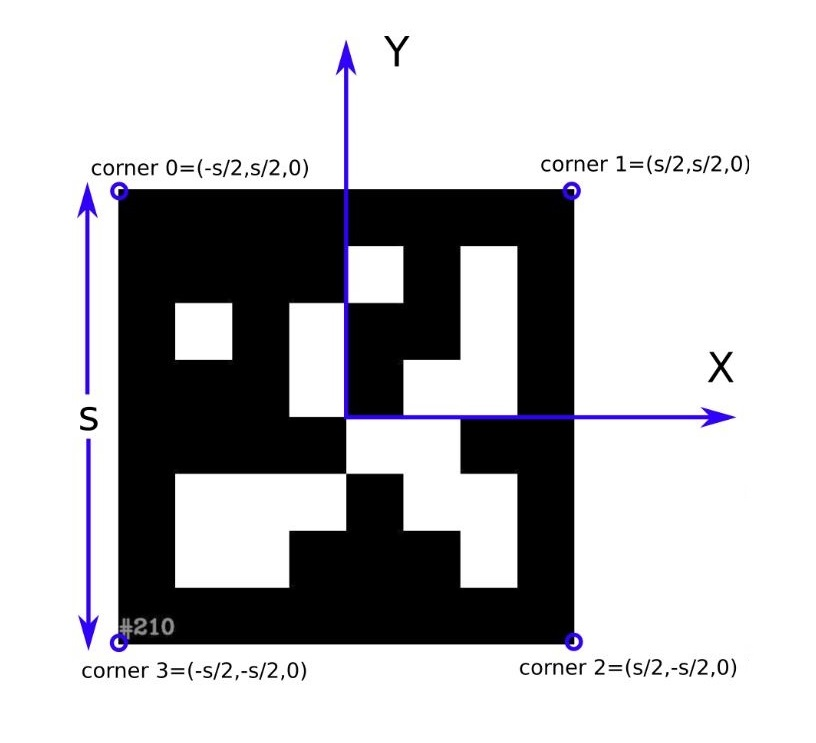
\includegraphics[width=10cm, height=10 cm]{figuras/aruco-identificador.jpg}
	\caption{Exemplo de erro de confusão entre marcadores,~\cite{Salinas2013}.}
	\label{fig:aruco-identificador}
\end{figure}

Segundo \citet{Salinas2013}, o processo de detecção do alvo ArUco inicia-se com a aplicação de um limiar adaptativo, de modo a obter as bordas. Em seguida são identificados os contornos dos alvos. Além dos alvos, são detectadas também várias bordas indesejadas. Estas bordas com pequeno número de pontos são eliminadas. Em seguida é realizada uma aproximação poligonal do contorno, de modo a manter os contornos côncavos com exatamente quatro cantos (retângulos). Então, os cantos são ordenados no sentido anti-horário e os retângulos muito próximos entre si são removidos, pois a detecção de bordas normalmente detecta a parte externa e interna da borda do marcador, preservando apenas a borda externa. Em seguida é tratada a perspectiva de projeção de modo a obter uma vista frontal da área de um retângulo, usando uma transformação projetiva. Usando o algoritmo de Otsu \cite{OTSU1979} e \cite{Artero2000}, assume-se uma distribuição bimodal e encontra-se o limiar que maximiza a variância extra-classe, mantendo uma baixa variação intra-classe. O marcador então é dividido numa grade 6x6, das quais as 25 células internas contém as informações de identificação. O resto corresponde à coroa externa. Inicialmente, verifica-se a presença da coroa. Em seguida, as 25 células internas são lidas para verificar se fornecem um código válido (pode ser necessário rotacionar o alvo para se obter um código válido). Caso seja um marcador válido, refinam-se os cantos usando uma técnica de interpolação sub-pixel.

%  Figura.
\begin{figure}[H]
	\centering
	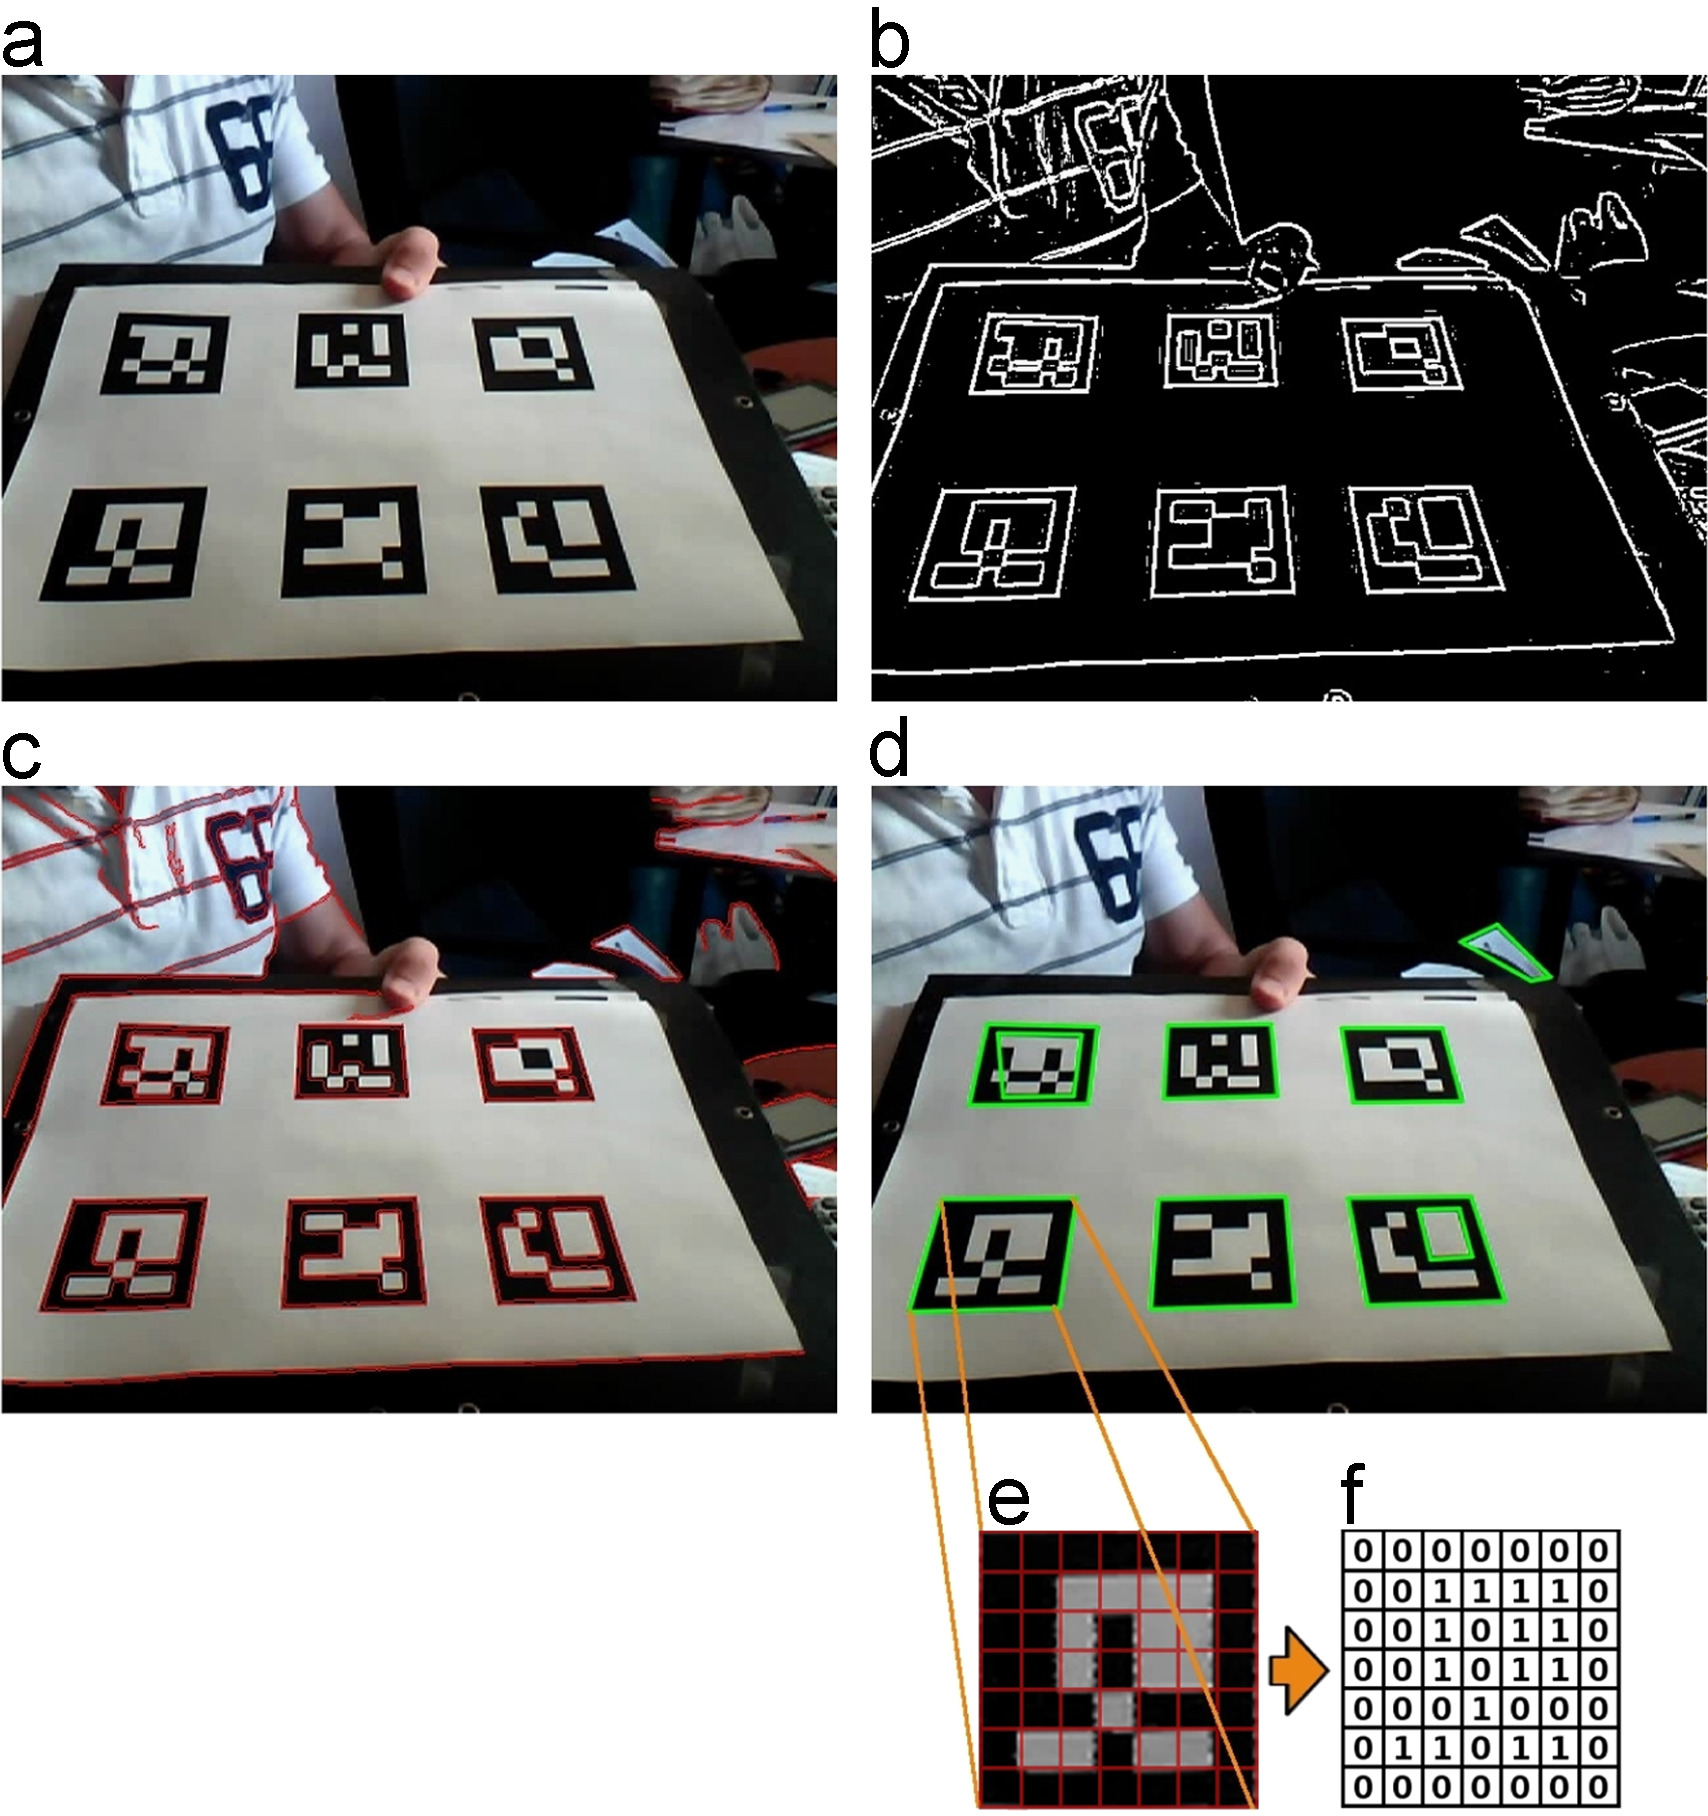
\includegraphics[width=12cm, height=12 cm]{figuras/aruco-processamento.jpg}
	\caption{Processamento de imagem para detecção automática de marcadores. (a) Imagem original. (b) Resultado da aplicação da limiarização local. c) Detecção de contornos. (d) Aproximação poligonal e remoção de contornos irrelevantes. (e) Exemplo de transformação de marcador após perspectiva. (f) Atribuição de bits para cada célula.,~\cite{Aruco2014}.}
	\label{fig:aruco-processamento}
\end{figure}

\section{\textit{Augmented Reality: Aruco 3}}

\textit{ArUco 3} é uma biblioteca de código aberto de realidade aumentada, criada para detectar marcadores fiduciais quadrados em imagens. Tendo a câmera devidamente calibrada, poderá ser estimado a pose da câmera em relação aos marcadores. A biblioteca é escrita em C++, mas há ferramentas para usar a biblioteca sem programação.

\section{Calibração de Câmera}

\subsection{Conceito}

\subsection{Projeção de Ponto 3D na Câmera}

\subsection{Calibração com ArUco}

\section{Estimação da Pose da Câmera com ArUco}

\section{Dicionário de Marcadores Proposto}

\section{Problemas de Detecção: Oclusão - Distorção - Falha em Longas Distâncias}

Um aspecto chave de tais dicionários é a distância inter-marcadores citada por \citet{Fiala2010}, que é a distância mínima de \textit{Hamming} entre os códigos binários dos marcadores, considerando as quatro rotações possíveis. Esta distância define o número máximo de \textit{bits} que podem ser corrigidos sem produzir um erro de confusão inter-marcadores, isto é, um marcador erroneamente identificado como diferente. Como consequência, a distância entre marcadores está diretamente relacionada aos recursos de correção de erros de um dicionário. Quanto maior o inter-marcador, menores as taxas de confusão de falso negativo e inter-marcadores e, portanto, maior a robustez do processo.

Por exemplo, a figura 1 mostra um exemplo de erro de confusão inter-marcadores e a importância de grandes distâncias inter-marcadores. Os dois primeiros marcadores têm uma curta distância de apenas 1 bit enquanto o terceiro marcador tem distâncias maiores de pelo menos 5  bits para o restante dos marcadores. Como pode ser visto na Figura ~\ref{fig:aruco-definicao} e, um único bit errôneo é suficiente para causar uma identificação errada do segundo marcador. Por outro lado, o terceiro marcador é identificado corretamente, apesar de ter um maior número de erros.

%  Figura.
\begin{figure}[h]
	\centering
	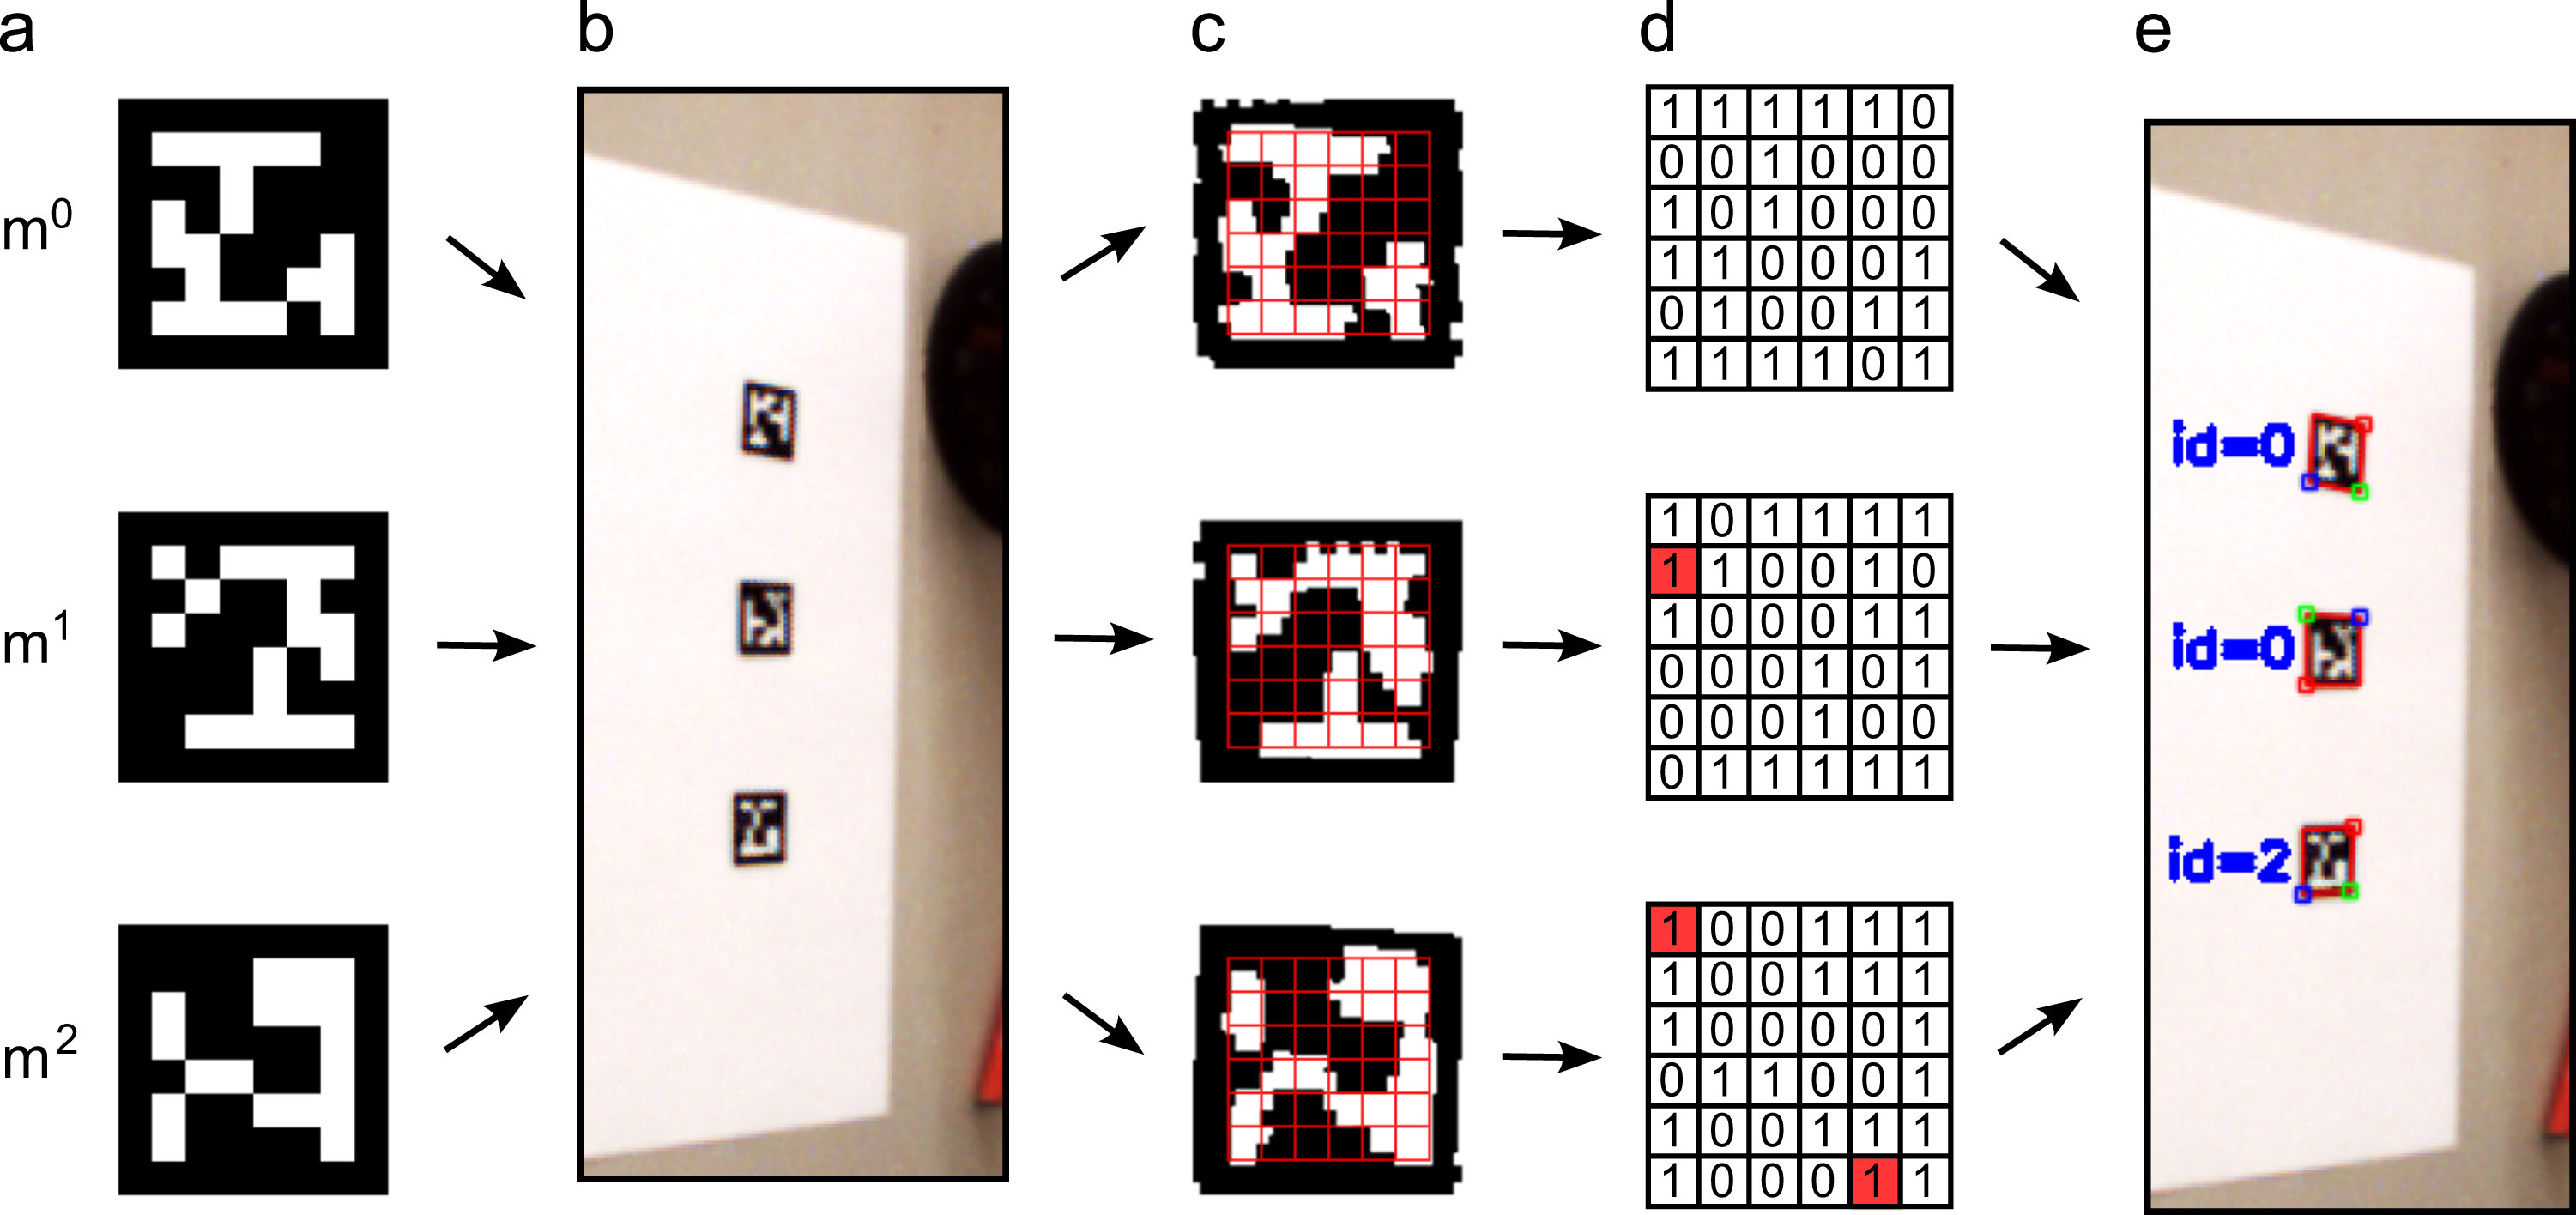
\includegraphics[width=14cm, height=6 cm]{figuras/arucofig1.jpg}
	\caption{Exemplo de erro de confusão entre marcadores,~\citet{Ramirez2018}.}
	\label{fig:aruco-definicao}
\end{figure}